\documentclass[12pt, french]{report}
\usepackage[utf8]{inputenc}
\usepackage[T1]{fontenc}
\usepackage{babel}

%additional packages
\usepackage{amsmath}
\usepackage{lipsum}
\usepackage{graphicx}
\usepackage{caption}
\usepackage{subcaption}
\usepackage{longtable}
\graphicspath{{figures/}}
\usepackage[a4paper,width=160mm,top=25mm,bottom=25mm]{geometry}
\usepackage{titlesec}
\linespread{1.2}

\usepackage{amsfonts,epsfig,cite,array,multirow,graphicx,amsmath,amsthm,ltablex,tabularx,setspace,arydshln,amssymb,multirow}
\usepackage{schemabloc,tikz}
\usetikzlibrary{circuits, arrows}

\newtheorem{theorem}{Theorem}
\newtheorem{lemma}{Lemma}
\usepackage[utf8]{inputenc}
\usepackage{amsmath}
\usepackage{amsfonts}
\usepackage{amssymb}
\usepackage{bbm}
\usepackage{mathtools}
\usepackage{textcomp}
\usepackage{stackengine}
\usepackage{booktabs}
\usepackage{longtable}
\usepackage{multirow}
\usepackage{graphicx}
\usepackage{epigraph}
\usepackage{minitoc}
\usepackage{blindtext}
\usepackage{hyperref}
\usepackage{float}



\title{\Huge{Loan Default Prediction}}
\author{Adjimon VITOFFODJI}
\date{Décembre 2024}
\def\mytitle{Loan Default Prediction}
\def\myname{Adjimon VITOFFODJI}
\def\degree{Master}
\def\mydegree{Mathématiques et Informatiques Appliqués aux Sciences Humaines et Sociales}
\def\mysupervisor{Sophie Lèbre}
\def\myrollno{17EE010XX}
\def\mydep{School of Electrical Sciences}



\begin{document}

%Front Matter
\dominitoc
 \pagenumbering{roman}
 % !TEX root = manuscript.tex
\begin{minipage}{.4\textwidth}
\begin{center}

\includegraphics[height=3cm]{logos/master.pdf}
\end{center}
\end{minipage}% This must go next to `\end{minipage}`
\hspace{2cm}
\begin{minipage}{.4\textwidth}
\begin{center}

\includegraphics[height=3cm]{logos/upv.eps}
\end{center}
\end{minipage}%


\begin{center}
\vspace{1cm}
{\huge UFR 6}\\
Université Paul Valéry, Montpellier III\\
\vspace{1cm}

{\Large Mémoire Professionnel S1M1}
\end{center}
\noindent\makebox[\linewidth]{\rule{\paperwidth}{0.4pt}}
\vspace{-20em}
{\let\newpage\relax\maketitle}
\vspace{-15em}
\noindent\makebox[\linewidth]{\rule{\paperwidth}{0.4pt}}

\begin{minipage}{.45\textwidth}

\end{minipage}% This must go next to `\end{minipage}`
\hspace{0.5cm}
\begin{minipage}{.45\textwidth}
\vspace{3em}
  
\end{minipage}
\newpage
 \addstarredchapter{Remerciements}
 % !TEX root = manuscript.tex
{\vspace*{8cm}\large
\section*{Remerciement}
\begin{itemize}
\item Je remercie mon professeur Sophie Lèbre pour avoir valider la thématique du projet.
\item Je remercie mon professeur M. Demangeot pour le cours de Classification supervisée et non supervisée.
\item Je remercie Sergei Shirkin Data Scientist at Dentsu Aegis pour avoir ouvert la compétition Loan Default Prediction. le jeu donnée mise à disposition qui a été une ressource essentielle pour ce projet. 
\end{itemize}
}
\newpage
 \addstarredchapter{Résumé}
 % !TEX root = manuscript.tex
\section*{Résumé}
La capacité à anticiper les défauts de paiement permet aux institutions financières non seulement de réduire les risques, mais aussi d'améliorer la rentabilité en ajustant les taux d'intérêt, en optimisant la gestion des créances et en affinant leur stratégie de prêt. En outre, l'intégration des modèles de machine learning dans ces processus promet une automatisation accrue et une prise de décision rapide et efficace.

Dans cette étude, nous avons exploré plusieurs modèles de machine learning pour résoudre un problème de classification, en utilisant la validation croisée pour évaluer leur performance de manière robuste. Les résultats ont révélé que certains modèles se distinguent clairement par leurs performances.

Le modèle de forêts aléatoires a montré les meilleurs résultats en termes d'accuracy, atteignant une moyenne de 0.7793 en validation croisée, et une performance stable sur les différents plis. Cela a confirmé la capacité de ce modèle à gérer des données complexes, à généraliser correctement, et à éviter le surapprentissage. À l'opposé, des modèles comme le SVM ont montré une performance relativement faible, ce qui suggère que le choix des hyperparamètres ou la nature des données pourrait ne pas être adapté à ce type de modèle.

En parallèle, l'analyse du F1-score macro, utilisé pour traiter le problème des classes déséquilibrées, a permis d'identifier le modèle de régression logistique comme le meilleur, avec un score moyen de 0.6462. Cette métrique a été cruciale pour équilibrer les performances sur les classes majoritaires et minoritaires, garantissant une évaluation plus juste des modèles dans un contexte de données déséquilibrées.

La validation croisée a joué un rôle clé en réduisant les risques d'overfitting et en nous permettant de mieux comprendre la stabilité et la fiabilité des différents modèles. Cependant, il est important de noter que même le modèle de forêts aléatoires, bien qu'efficace sur l'ensemble d'entraînement, présente des limites sur le rappel de la classe minoritaire, ce qui pourrait être amélioré par l'ajustement des hyperparamètres ou l'utilisation d'approches spécifiques pour gérer le déséquilibre des classes.

Enfin, bien que la régression logistique ait été sélectionnée comme le meilleur modèle pour le F1-score macro, l'amélioration continue des performances reste possible en ajustant les paramètres et en explorant d'autres techniques de prétraitement et de pondération des classes. Cette étude met en lumière l'importance de choisir les bons modèles et les bonnes métriques en fonction des caractéristiques spécifiques des données et des objectifs de la tâche.


\newpage


\tableofcontents
\addstarredchapter{Liste des figures}
\listoffigures
\addstarredchapter{Liste des tables}
\listoftables
%Chapters
\clearpage
\pagenumbering{arabic}

\addstarredchapter{Introduction}
% !TEX root = manuscript.tex
\chapter*{Introduction}

La prédiction du défaut de crédit est une tâche importante dans le domaine de la finance, car elle permet aux institutions financières de mieux évaluer le risque associé à chaque emprunt. Une prédiction précise peut aider à prendre des décisions éclairées sur l'octroi de crédits et à minimiser les pertes potentielles.

Dans le cadre de cette compétition Kaggle intitulée "Loan Default Prediction" organisée par Sergei Shirkin, le défi consiste à prédire si un emprunteur fera défaut sur un prêt en utilisant un jeu de données de caractéristiques financières. L'objectif principal de cette compétition est de développer un modèle capable de prédire la probabilité de défaut de crédit à partir des informations disponibles dans un jeu de données d'entraînement. Le jeu de données train.csv contient diverses caractéristiques des emprunteurs ainsi que la variable cible, "Credit Default", tandis que le jeu de données test.csv ne contient que les caractéristiques des emprunteurs, pour lesquels les prédictions doivent être faites.

Ce rapport présente l'approche adoptée pour résoudre ce problème de classification binaire, ainsi que les différentes étapes entreprises, telles que l'exploration des données, le prétraitement, la modélisation et l'évaluation des performances. L'évaluation du modèle est réalisée à l'aide de la métrique F1 score, qui équilibre la précision et le rappel, offrant une évaluation robuste de la performance du modèle sur des classes déséquilibrées.

Le défi propose une opportunité d'améliorer les compétences en machine learning, en particulier dans le domaine de la classification des risques, tout en mettant en pratique des techniques d'analyse de données, de sélection de caractéristiques et de validation de modèles.


% !TEX root = manuscript.tex

\chapter{Nettoyage, Exploration et Analyse descriptive des données}
\minitoc
\newpage
\section{Nettoyage et Analyse du jeu de données train}


\subsection{Statistique descriptive des données train }
Le jeu de donnée d'entrainement (train), dispose de 7500 lignes et 18 colonnes. L'analyse descriptive (voir figure \ref{fig:stat_descriptive}) de ce dernier nous montre que les colonnes Annual Income, Months since last delinquent, Credit Score et Years in current qui contiennent plusieurs valeurs manquantes(Na). Par la suite, nous avons utilisé la médiane pour la gestion des valeurs manquantes. 

\begin{figure}[H]
\centering
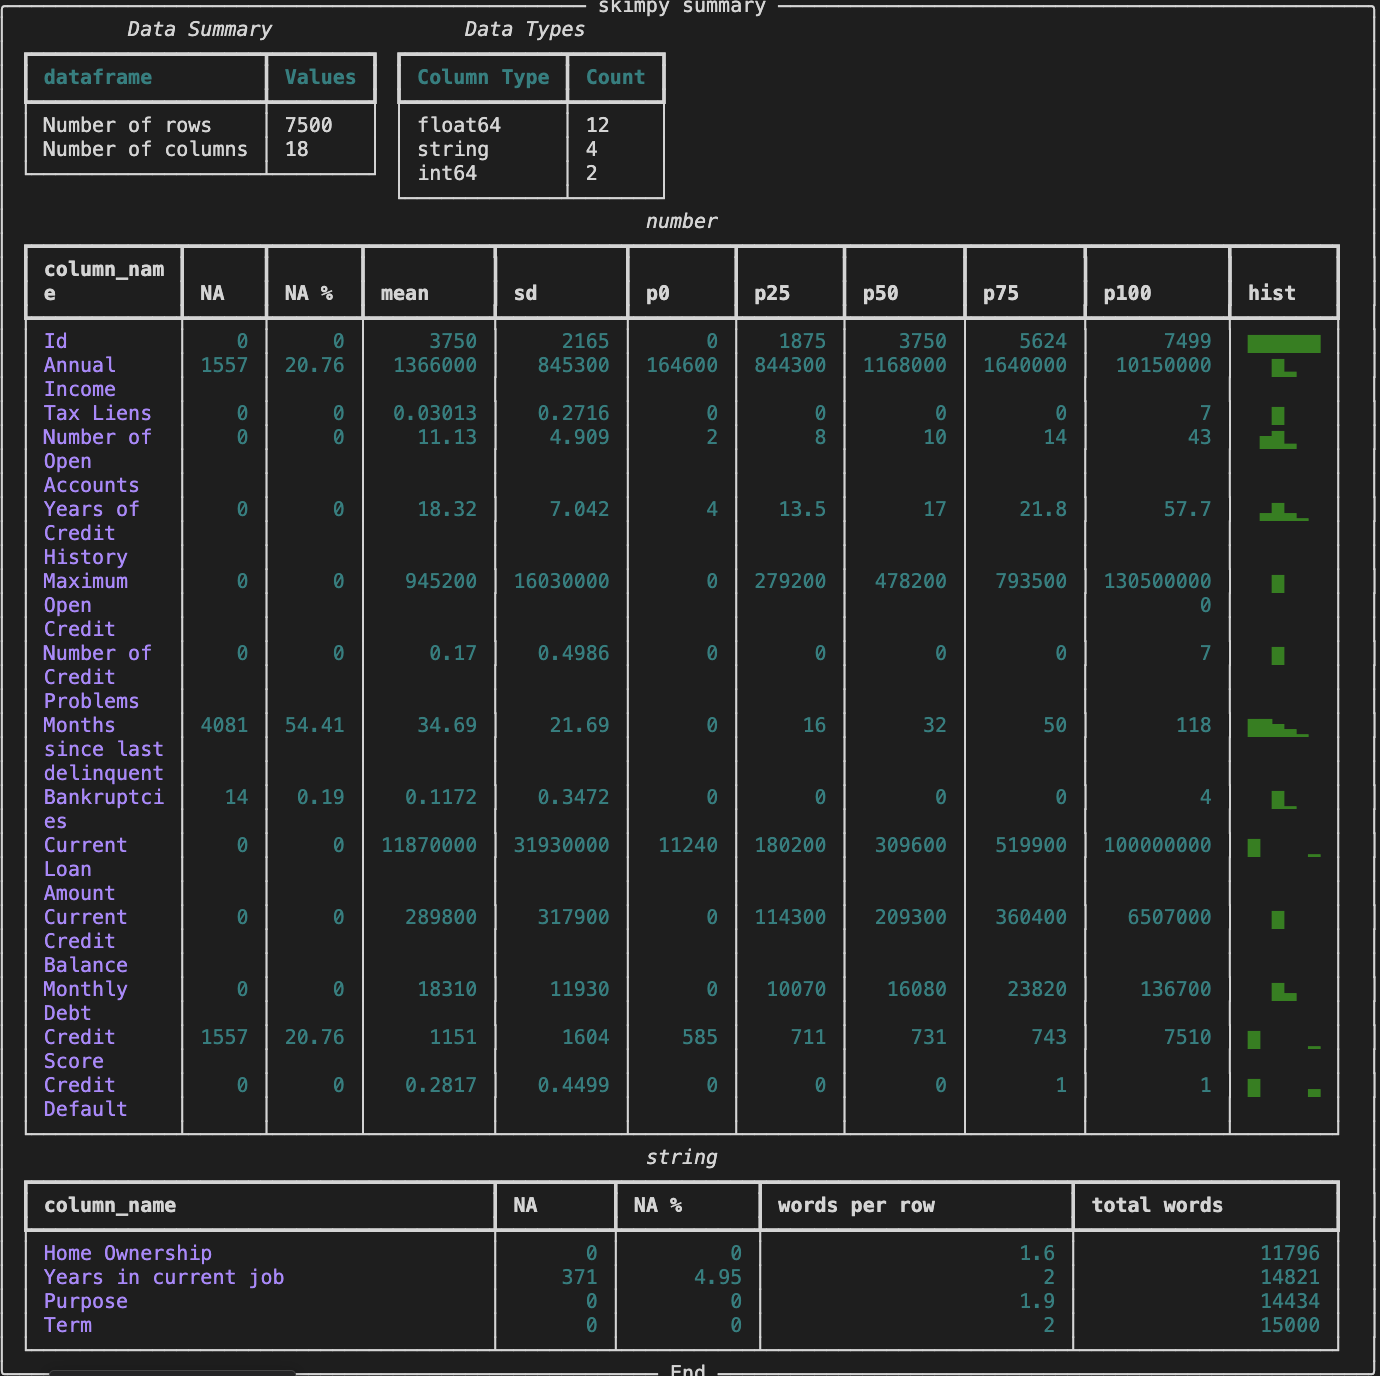
\includegraphics[width=0.8\textwidth]{figures/fig1.png}
\caption{Statistique descriptive train.}
\label{fig:stat_descriptive}
\end{figure}

\subsection{Matrice de corrélation}
\begin{flushleft}
\begin{enumerate}
\item Nous allons dans un premier temps représenter la matrice de corrélation avec les colonnes numériques(voir figure \ref{fig:matrice_corr}). 
\begin{flushleft}
On note une très faible correlation linéaire entre le Credit Default et les autre variables quantitative.

De même, on note d'une part une faible liaison négative entre Credit Default et Current Loan Amont et d'autre part une faible liaison postive entre Credit Default et Credit Score

Certaines colonnes ont des corrélations très faibles (proches de 0), ce qui peut indiquer qu'elles n'ont pas d'impact direct sur Credit Default.
\end{flushleft} 

\begin{figure}[H]
\centering
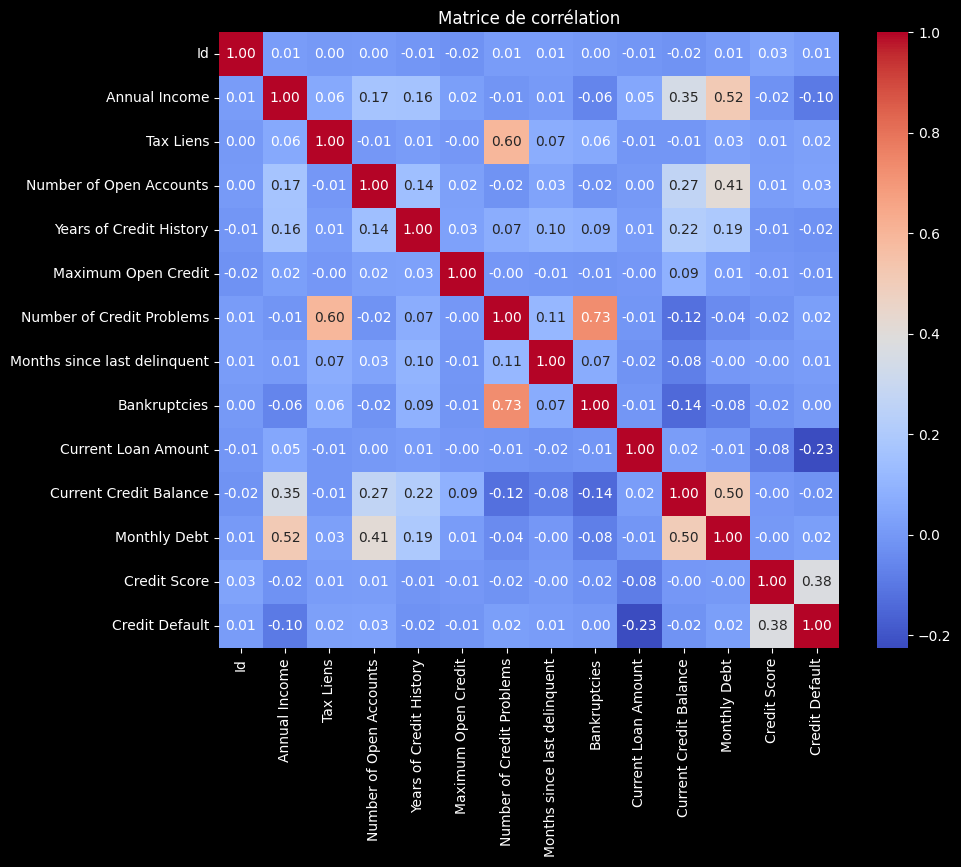
\includegraphics[width=0.8\textwidth]{figures/Matrice1.png}
\caption{Matrice de corrélation.}
\label{fig:matrice_corr}
\end{figure}


\item Par la suite, nous avons utilisé la technique d'encodage \textbf{LabelEncoder} pour encoder la colonne \textbf{Years in current job}, puis avons utilisé \textbf{One-Hot Encoding} pour encoder les autres colonnes catégorielles. 
\end{enumerate}
\end{flushleft}
\begin{flushleft}

La corrélation la plus élevée avec Credit Default est pour Credit Score (0.44), ce qui peut indiquer une relation modérée entre ces deux variables.
Term\_Long Term et Term\_Short Term ont des corrélations opposées (0.181 et -0.181), ce qui est logique car elles sont mutuellement exclusives dans un encodage one-hot.

Certaines colonnes ont des corrélations très faibles (proches de 0), ce qui peut indiquer qu'elles n'ont pas d'impact direct sur Credit Default.


Pour soumettre notre jeu de données train aux différents modèles de classification, nous avons besoin de convertir nos colonnes issues du \textbf{pd.get\_dummies()} en de type \textbf{int}, cela facilitera leur traitement dans certains modèles ou calculs. Par la suite nous allons normaliser les colonnes pour éviter les biais dus à des échelles différentes. (Voir le résumé statistique après analyse et traitement des données à l'annexe Annexe~\ref{sec:annexe3}).
\end{flushleft}

\section{Nettoyage et Analyse du Jeu de donnée test}
\subsection{Statistiques descriptives}

Le jeu de donnée d'entrainement (train), dispose de 2500 lignes et 17 colonnes. L'analyse descriptive (voir figure \ref{fig:stats_descriptive}) de ce dernier nous montre que les colonnes Annual Income, Months since last delinquent, Credit Score et Years in current qui contiennent plusieurs valeurs manquantes(Na). Par la suite, nous avons utilisé la médiane pour la gestion des valeurs manquantes. (voir Annexe~\ref{sec:annexe4}).

\begin{figure}[H]
\centering
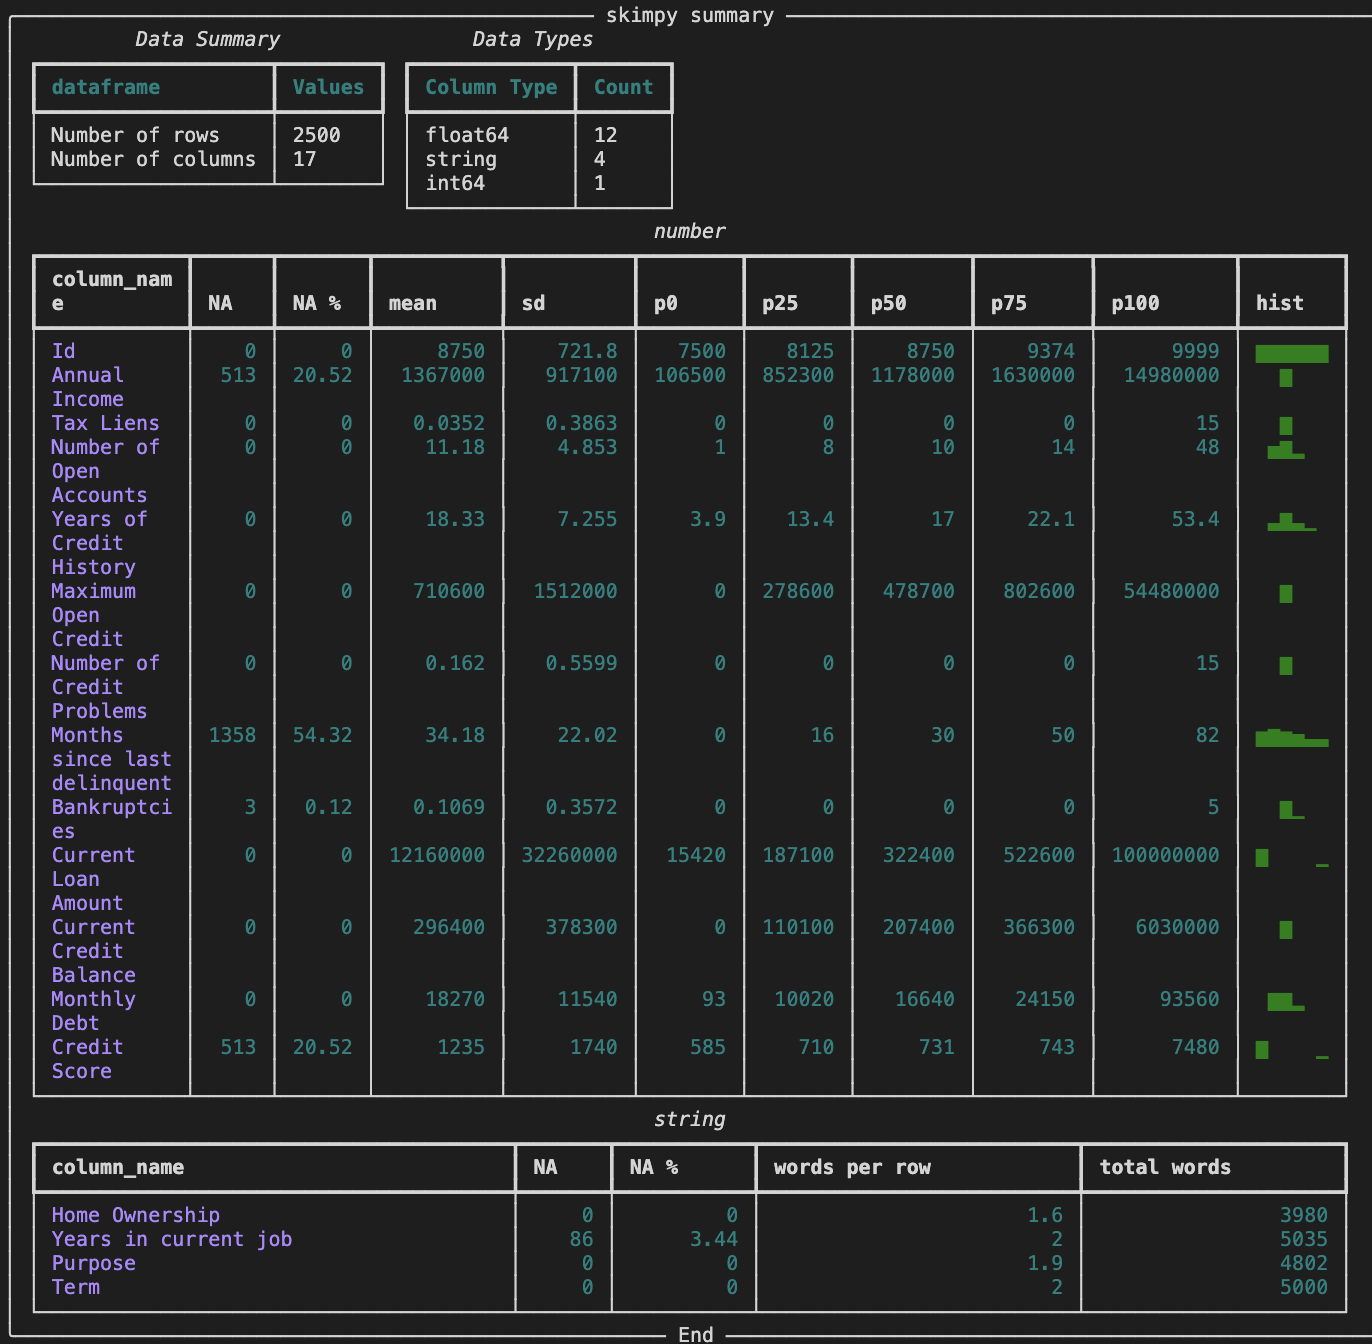
\includegraphics[width=0.8\textwidth]{figures/fig2.png}
\caption{Statistique descriptive test.}
\label{fig:stats_descriptive}
\end{figure}


\subsection{Traitement du jeu de donnée test}

Nous avons utilisé les mêmes techniques de nettoyage, de normalisation, de standardisation et d'encodage sur le jeu de donnée test. (voir le résumé statistique après nettoyage à l'annexe Annexe~\ref{sec:annexe4}). 


% !TEX root = manuscript.tex

\chapter{Entrainement des modèles et interprétation des résultats }
\epigraph{ Nous avons divisé les données(train), en données d'entraînement et de validation.}{}
\minitoc
\newpage
\section{Entrainement des modèles}
\subsection{Arbre de décision}
\begin{flushleft}
\begin{enumerate}
\item Accuracy (Précision globale)
Accuracy = 0.7627

Cela signifie que 76,27\% des prédictions du modèle sont correctes. C'est la proportion des prédictions correctes (que la prédiction soit pour la classe 0 ou 1) parmi l'ensemble des prédictions réalisées. Cependant, l'accuracy peut être trompeuse si les classes sont déséquilibrées. Ce qui est le cas ici.

\item Métriques pour chaque classe

Classe 0 (la classe majoritaire dans ce cas)
Precision = 0.78 :
Sur toutes les prédictions faites comme étant de la classe 0, 78\% étaient correctes. Autrement dit, si le modèle prédit que l'observation appartient à la classe 0, il a 80\% de chances de faire une prédiction correcte.

Recall = 0.92 :
Parmi toutes les vraies instances de la classe 0, 92\% ont été correctement identifiées par le modèle. Cela indique que le modèle est assez bon pour identifier la classe 0, mais il y a encore 8\% des exemples de la classe 0 qui sont manqués.

F1-score = 0.85 :
Le F1-score est une moyenne harmonique entre la precision et le recall. C'est une métrique utile quand on veut un compromis entre les deux, particulièrement dans des contextes où l'on veut éviter à la fois de fausses alertes (fausses positives) et des faux négatifs. Ici, le modèle montre un bon équilibre pour la classe 0.

Classe 1 (la classe minoritaire)

Precision = 0.67 : 
Sur toutes les prédictions faites comme étant de la classe 1, 67 \% étaient correctes. Le modèle semble avoir plus de mal à prédire correctement la classe 1 que la classe 0.

Recall = 0.39 :
Parmi toutes les vraies instances de la classe 1, 39\% ont été correctement identifiées. Cela suggère que le modèle a des difficultés à reconnaître la classe 1, et il manque 61 \% des exemples de cette classe.

F1-score = 0.49 :
L'F1-score pour la classe 1 est relativement faible, ce qui reflète une combinaison de précision et de rappel qui n'est pas idéale. Cela montre que le modèle a un équilibre défavorable pour cette classe.

\item Métriques moyennes (macro et weighted avg):

Macro avg :

Precision = 0.72, Recall = 0.65, F1-score = 0.67 :
Ces valeurs sont les moyennes des métriques pour les deux classes, calculées sans tenir compte du déséquilibre des classes. La macro moyenne donne une idée générale de la performance du modèle sur toutes les classes, indépendamment de leur fréquence dans les données.


Weighted avg :

Precision = 0.75, Recall = 0.76, F1-score = 0.74 :
La weighted moyenne prend en compte la fréquence des classes dans le dataset (plus de 5000 instances de la classe 0 contre environ 2100 pour la classe 1). Ces valeurs montrent qu'en pondérant par la taille des classes, le modèle est un peu plus performant sur la classe 0, mais reste assez équilibré.

En conclusion:

Le modèle est globalement performant, mais il a un déséquilibre de performance entre les deux classes. 

Il fait un très bon travail pour prédire la classe 0, avec une précision élevée (78\%) et un rappel élevé (92\%).

Cependant, il a plus de mal avec la classe 1, avec un rappel faible (39\%) et un F1-score assez bas (49\%), ce qui suggère que le modèle manque beaucoup de cas positifs pour cette classe.

Cela pourrait être dû à un déséquilibre de classes (plus d'exemples de la classe 0 que de la classe 1)
\end{enumerate}
\end{flushleft}

\begin{table}[H]
\centering
\caption{Résultats de performance sur les données de validation-Arbre de décision}
\label{tab:performance_Arbre}
\begin{tabular}{|l|c|c|c|c|}
\hline
\textbf{Classe}     & \textbf{Precision} & \textbf{Recall} & \textbf{F1-Score} & \textbf{Support} \\ \hline
0                   & 0.78               & 0.92            & 0.85              & 1059             \\ \hline
1                   & 0.67               & 0.39            & 0.49              & 441              \\ \hline
\textbf{Accuracy}   & \multicolumn{2}{|c|}{} & 0.76 &  1500                              \\ \hline
\textbf{Macro Avg}  & 0.72               & 0.65            & 0.67              & 1500             \\ \hline
\textbf{Weighted Avg} & 0.75               & 0.76            & 0.74              & 1500             \\ \hline
\end{tabular}
\begin{flushleft}
Accuracy sur les données de validation: 0.7626666666666667
\end{flushleft}
\end{table}

\begin{figure}[H]
\centering
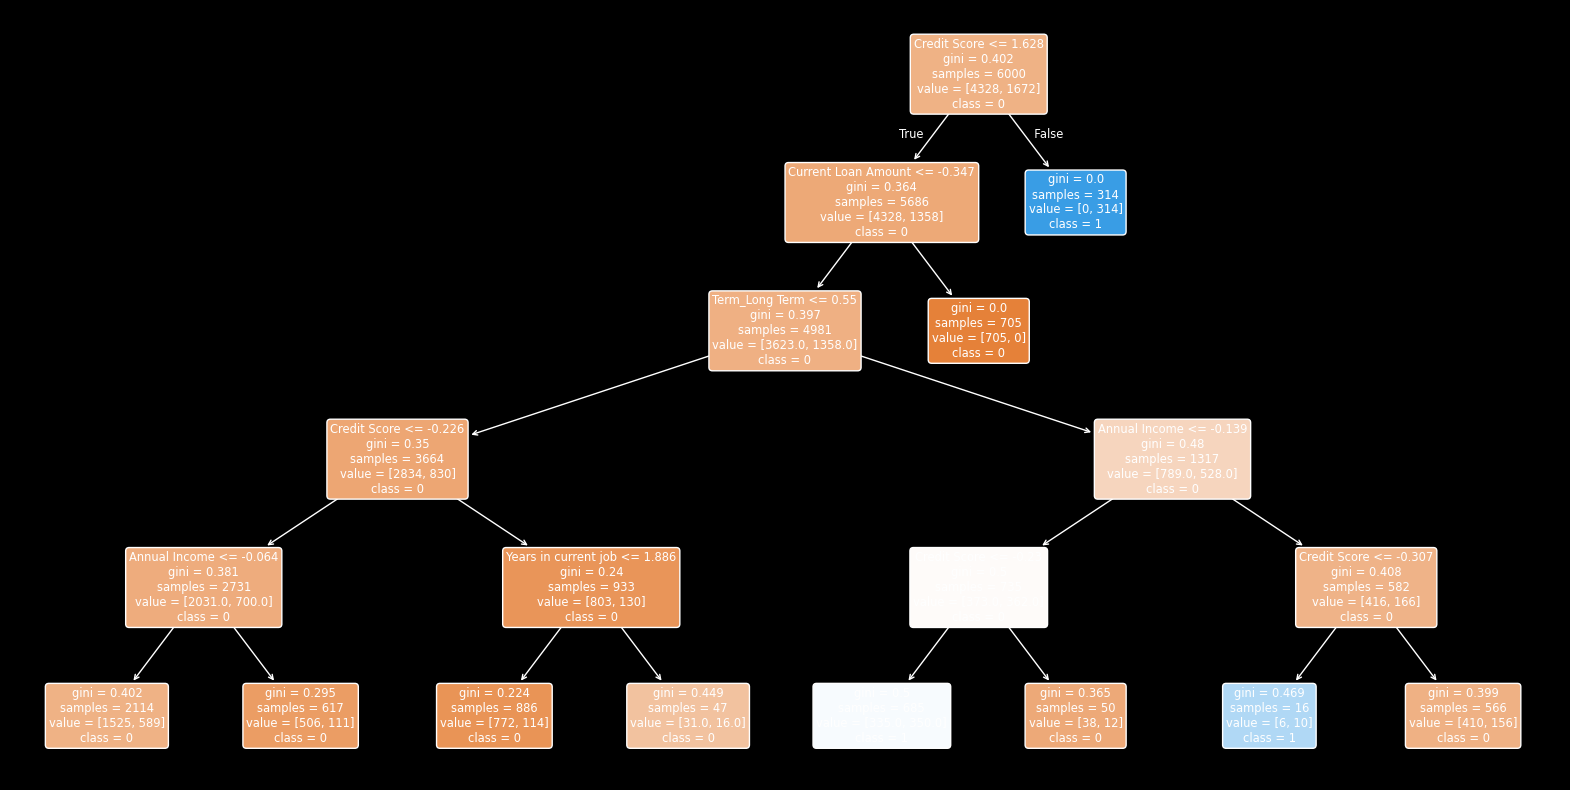
\includegraphics[width=1\textwidth]{figures/arbre.png}
\caption{arbre de décision.}
\label{fig:arbre_deci}
\end{figure}


\begin{flushleft}
La matrice de confusion et la courbe de ROC (voir Annexe~\ref{sec:annexe5}) indiquent que le modèle a une bonne capacité à distinguer entre les classes, mais il n'est pas parfait.
\end{flushleft}



\subsection{Régression logistique}
\begin{flushleft}
\begin{enumerate}
\item Accuracy : 76.6\%

L'accuracy mesure la proportion globale des prédictions correctes. Ici, le modèle prédit correctement 76,6 \% des cas. Bien que ce soit un bon résultat, ce chiffre seul ne suffit pas à évaluer la performance du modèle, surtout si les classes sont déséquilibrées. Ce qui est le cas ici.

\item Precision, Recall et F1-Score pour la classe 0 (Non-défaillant) :

Precision = 0.76 : Cela signifie que parmi toutes les prédictions faites par le modèle comme étant "0" (non défaut), 76\% étaient correctes.

Recall = 0.98 : Cela signifie que parmi tous les vrais cas "0", le modèle a réussi à en prédire 98\%. Cela indique que le modèle est très bon pour détecter les non-défaillants.

F1-Score = 0.86 : Le F1-score est une moyenne harmonique entre la précision et le rappel, donc ici, il est relativement élevé, ce qui signifie que le modèle a une bonne capacité à détecter les cas de "0" tout en minimisant les faux positifs.

\item Precision, Recall et F1-Score pour la classe 1 (Défaillant) :

Precision = 0.85 : Cela signifie que parmi toutes les prédictions faites par le modèle comme étant "1" (défaut), 85\% étaient correctes.

Recall = 0.25 : Ici, seulement 25\% des vrais cas "1" ont été détectés. C'est un faible score, ce qui signifie que le modèle a du mal à identifier les clients en défaut.

F1-Score = 0.38 : Ce score est également faible, ce qui reflète une mauvaise performance du modèle pour prédire les défauts

\item Macro et Weighted Averages :

Macro avg : Cela donne une moyenne simple des scores de chaque classe (sans tenir compte de la proportion des classes), ce qui donne un score de 0.80 pour la précision, 0.62 pour le rappel et 0.63 pour le F1-score.

Weighted avg : Cette moyenne prend en compte la distribution des classes. Ici, la précision et le rappel sont équilibrés à 0.79 et 0.77 respectivement, avec un F1-score global de 0.72.

En conclusion:
Le modèle est globalement performant, mais faible déséquilibre de performance entre les deux classes.
\end{enumerate}
\end{flushleft}

\begin{table}[H]
\centering
\caption{Résultats de performance sur les données de validation-Régression Logistique}
\label{tab:performance_validation_RegL}
\begin{tabular}{|l|c|c|c|c|}
\hline
\textbf{Classe}       & \textbf{Precision} & \textbf{Recall} & \textbf{F1-Score} & \textbf{Support} \\ \hline
0                     & 0.76               & 0.98            & 0.86              & 1059             \\ \hline
1                     & 0.85               & 0.25            & 0.38              & 441              \\ \hline
\textbf{Accuracy} & \multicolumn{2}{|c|}{} & 0.77       & 1500     \\ \hline
\textbf{Macro Avg}    & 0.80               & 0.61            & 0.62              & 1500             \\ \hline
\textbf{Weighted Avg} & 0.79               & 0.77            & 0.72              & 1500             \\ \hline
\end{tabular}
\begin{flushleft}
Accuracy sur les données de validation: 0.766
\end{flushleft}
\end{table}

\begin{flushleft}
La matrice de confusion et la courbe de ROC associées (voir Annexe~\ref{sec:annexe6}) indiquent que le modèle a une performance acceptable à distinguer entre les deux classes. 
\end{flushleft}

\subsection{Forêt aléatoire}
\begin{flushleft}
\begin{enumerate}

\item Accuracy (Précision globale) :
L'accuracy est de 76.33\%, ce qui signifie que 76.33\% des prédictions du modèle sont correctes sur l'ensemble de validation. Cependant, cette métrique seule peut être trompeuse si les classes sont déséquilibrées.

\item Métriques pour chaque classe :

Classe 0 (support : 1059 instances) :

Précision (Precision) = 0.76 : 
Cela signifie que, parmi les prédictions de la classe 0, 76\% étaient correctes.

Rappel (Recall) = 0.96 : 
Cela signifie que le modèle a identifié 96\% des instances appartenant réellement à la classe 0.

F1-score = 0.85 : 
Le modèle a bien équilibré précision et rappel pour la classe 0, montrant une bonne performance.

Classe 1 (support : 441 instances)  :

Précision (Precision) = 0.76 :
Cela signifie que, parmi les prédictions de la classe 1, 76\% étaient correctes.

Rappel (Recall) = 0.29 :
Cela signifie que le modèle n'a identifié que 29\% des instances appartenant réellement à la classe 1.

Problème notable : Le modèle a de grandes difficultés à détecter la classe 1.

F1-score = 0.42 :
Un faible F1-score montre que le modèle est déséquilibré dans sa capacité à prédire correctement la classe 1.

\item Macro Avg (Moyenne non pondérée) :

Précision, Rappel, F1-score :
Ces moyennes prennent en compte les métriques de chaque classe avec un poids égal.

Précision moyenne = 0.76; Rappel moyen = 0.62; F1-score moyen = 0.63.
Cela montre que, en moyenne, les performances du modèle sont limitées par sa faible capacité à gérer la classe 1.


\item Weighted Avg (Moyenne pondérée par le support):
Ces moyennes tiennent compte de l'importance relative des classes (plus de poids pour la classe 0, qui a plus d'exemples).

Précision pondérée = 0.76; Rappel pondéré = 0.76; F1-score pondéré = 0.72. 
Ces scores montrent que les performances globales semblent correctes, mais elles sont biaisées par la bonne performance sur la classe majoritaire (classe 0).

En résumé:

Le modèle Random Forest montre une bonne capacité à identifier la classe majoritaire (classe 0), mais il a des difficultés à prédire la classe minoritaire (classe 1).
\end{enumerate}
\end{flushleft}

\begin{table}[H]
\centering
\caption{Résultats de performance sur les données de validation Forêt aléatoire}
\label{tab:performance_validation_FoAl}
\begin{tabular}{|l|c|c|c|c|}
\hline
\textbf{Classe}       & \textbf{Precision} & \textbf{Recall} & \textbf{F1-Score} & \textbf{Support} \\ \hline
0                     & 0.76               & 0.96            & 0.85              & 1059             \\ \hline
1                     & 0.76               & 0.29            & 0.42              & 441              \\ \hline
\textbf{Accuracy} & \multicolumn{2}{|c|}{} & 0.76            & 1500     \\ \hline
\textbf{Macro Avg}    & 0.76               & 0.62            & 0.63              & 1500             \\ \hline
\textbf{Weighted Avg} & 0.76               & 0.76            & 0.72              & 1500             \\ \hline
\end{tabular}
\begin{flushleft}
Accuracy sur les données de validation: 0.763
\end{flushleft}
\end{table}




\begin{flushleft}
La matrice de confusion et la courbe de ROC associées (voir Annexe~\ref{sec:annexe7}) indiquent que (l'AUC = 0.76) le modèle a performance acceptable à distinguer entre les deux classes.
\end{flushleft}
 
\subsection{Support Vector Machines (SVM)}
\begin{flushleft}
\begin{enumerate}
\item Accuracy (Précision globale): 0.452
L'accuracy est de 45,2\%, ce qui signifie que le modèle fait des prédictions correctes environ 45\% du temps.

\item Métriques pour chaque classe

Pour la classe 0 :

La précision de la classe 0 est assez bonne, ce qui signifie que, parmi toutes les prédictions où le modèle a dit classe 0, 71\% étaient correctes.

Le rappel pour la classe 0 est assez faible, ce qui signifie que parmi toutes les instances réelles de la classe 0, le modèle n'a réussi à en identifier que 38\%.

Le F1-score(0.50) pour la classe 0 est relativement moyen, ce qui reflète un compromis entre la précision et le rappel.

Pour la classe 1 :

Précision de  0.29 (29\%) : La précision de la classe 1 est faible, ce qui signifie qu'une grande proportion des prédictions de la classe 1 étaient incorrectes.


Recall de  0.62 (62\%): Le rappel pour la classe 1 est meilleur, ce qui signifie que le modèle a identifié 62\% des instances réelles de cette classe.

F1-score de 0.40 : Le F1-score pour la classe 1 est plus faible, ce qui indique que le modèle lutte davantage pour classer correctement les instances de cette classe.

Déséquilibre des classes :

Le déséquilibre des classes explique en grande partie cette performance biaisée. Le modèle est plus performant pour prédire la classe majoritaire (classe 0), ce qui conduit à des performances médiocres pour la classe minoritaire (classe 1). Cela se traduit par un recall faible pour la classe 1 et un biais vers la prédiction de la classe 0.

En résumé:

Le modèle SVM ne semble pas très performant, particulièrement pour la classe minoritaire (1). Il fait mieux sur la classe majoritaire (0) mais il est relativement mauvais pour détecter les instances de la classe 1.
\end{enumerate}
\end{flushleft}

\begin{table}[H]
\centering
\caption{Résultats de performance sur les données de validation - SVM}
\label{tab:performance_validation_SVM}
\begin{tabular}{|l|c|c|c|c|}
\hline
\textbf{Classe}       & \textbf{Precision} & \textbf{Recall} & \textbf{F1-Score} & \textbf{Support} \\ \hline
0                     & 0.71               & 0.38            & 0.50              & 1059             \\ \hline
1                     & 0.29               & 0.62            & 0.40              & 441              \\ \hline
\textbf{Accuracy} & \multicolumn{2}{|c|}{} & 0.45       & 1500     \\ \hline
\textbf{Macro Avg}    & 0.50               & 0.50            & 0.45              & 1500             \\ \hline
\textbf{Weighted Avg} & 0.59               & 0.45            & 0.47              & 1500             \\ \hline
\end{tabular}
\begin{flushleft}
Accuracy sur les données de validation: 0.452
\end{flushleft}
\end{table}


\begin{flushleft}
La matrice de confusion et la courbe de ROC associées (voir Annexe~\ref{sec:annexe8}) indiquent que (l'AUC=0.51) le modèle ne parvient pas à mieux prédire que de simples prédictions aléatoires.
\end{flushleft}
 
\subsection{K Nearest Neighbors (KNN)}
\begin{flushleft}
\begin{enumerate}

\item Accuracy (Précision globale): 0.699 (~7\%)

L'accuracy est de 0.699 (~70\%), indique que le modèle prédit correctement 70\% des échantillons de validation. Cependant, l'accuracy seule peut être trompeuse, en particulier si les classes sont déséquilibrées (ce qui semble être le cas ici)

\item Métrique pour les classes

Pour la classe 0 :

Précision (Precision) = 0.70. Cela signifie que, parmi toutes les prédictions faites comme étant de la classe 0, 70\% étaient correctes.

Rappel (Recall) = 0.99. Cela signifie que 99\% des instances de la classe 0 ont été correctement identifiées par le modèle. Le modèle est donc très performant pour la classe 0.

F1-Score = 0.82. Une bonne combinaison de la précision et du rappel pour la classe 0. Le modèle fait bien pour la classe majoritaire.

Pour la classe 1 :

Précision (Precision) = 0.14. Parmi les prédictions faites comme étant de la classe 1,seulement 14\% étaient correctes.

Rappel (Recall) = 0.00. Le modèle n'a pratiquement pas réussi à identifier les instances réelles de la classe 1 (seules quelques-unes, voire aucune, ont été correctement classées)

F1-Score = 0.01. La combinaison de la précision et du rappel est faible, ce qui indique que la classe 1 est mal prédite.

\item Moyennes(sans pondération des effectifs) Macro avg :

La macro-moyenne montre des résultats faibles (~0.42 pour F1-score), en raison des mauvaises performances sur la classe 1.

\item Weightedtenant compte de la proportion des instances dans chaque classe() avg :

Avec une pondération pour la classe majoritaire (classe 0), les scores sont légèrement meilleurs (~0.58 pour F1-score), mais toujours médiocres.

Déséquilibre des classes :

Le déséquilibre des classes explique en grande partie cette performance biaisée. Le modèle est plus performant pour prédire la classe majoritaire (classe 0), ce qui conduit à des performances médiocres pour la classe minoritaire (classe 1). Cela se traduit par un recall faible pour la classe 1 et un biais vers la prédiction de la classe 0.

En résumé:

En résumé, le modèle KNN avec K=20 montre de bonnes performances pour la classe 0 (majoritaire), mais échoue à prédire la classe 1 (minoritaire).
\end{enumerate}
\end{flushleft}

\begin{table}[H]
\centering
\caption{Résultats de performance pour KNN avec K=20 sur les données de validation}
\label{tab:knn_k20_validation}
\begin{tabular}{|l|c|c|c|c|}
\hline
\textbf{Classe}       & \textbf{Precision} & \textbf{Recall} & \textbf{F1-Score} & \textbf{Support} \\ \hline
0                     & 0.70               & 0.99            & 0.82              & 1059             \\ \hline
1                     & 0.14               & 0.00            & 0.01              & 441              \\ \hline
\textbf{Accuracy} & \multicolumn{2}{|c|}{} & 0.70    & 1500     \\ \hline
\textbf{Macro Avg}    & 0.42               & 0.50            & 0.42              & 1500             \\ \hline
\textbf{Weighted Avg} & 0.54               & 0.70            & 0.58              & 1500             \\ \hline
\end{tabular}
\begin{flushleft}
Meilleur nombre de voisins (\textbf{K}): 20 \\
Accuracy sur les données de validation: 0.699.
\end{flushleft}
\end{table}


\begin{flushleft}
La matrice de confusion et la courbe de ROC associées (voir Annexe~\ref{sec:annexe9}) indiquent : Bien que le modèle ait un AUC relativement supérieur à 0.5, cela suggère qu'il n'est pas très bon pour séparer les classes, en particulier dans un cas de classe déséquilibrée. 
le modèle ne parvient pas à mieux prédire que de simples prédictions aléatoires.
\end{flushleft}

\section{Comparaison et Validation croisée}
\subsection{Comparaison et Validation croisée avec Accuracy}
\begin{flushleft}
Les résultats de la validation croisée montrent la moyenne d'accuracy pour chaque modèle sur les 5 plis. Ces scores aident à évaluer la stabilité et la performance générale des modèles, tout en réduisant les risques de sur-apprentissage (overfitting).

\begin{enumerate}
\item Précision globale
\begin{itemize}
\item Arbre de décision (Accuracy moyenne = 0.6908) : L'arbre de décision a une performance correcte.
Performance moyenne, avec une forte variation entre les folds (de 0.6791 à 0.6991). Cela indique que l’arbre de décision est sensible aux variations dans les données d’entraînement, probablement dû à un surapprentissage (overfitting) dans certains cas.
\item Régression logistique (Accuracy moyenne = 0.6872) : La régression logistique montre une performance stable, mais légèrement inférieure à celle des forêts aléatoires.  C'est un modèle linéaire, donc il pourrait être limité si les relations entre les variables ne sont pas linéaires.
\item Forêts aléatoires (Accuracy moyenne = 0.7793) :
C'est clairement le modèle le plus performant en validation croisée. Il combine plusieurs arbres de décision pour améliorer la généralisation et réduire le surapprentissage. La faible variance entre les plis confirme qu'il s'adapte bien aux données.
\item SVM (Accuracy moyenne = 0.5130) : Le SVM affiche des performances très faibles.
Cela pourrait être dû à des hyperparamètres non optimaux ou à un déséquilibre dans les classes.
\item KNN (Accuracy moyenne = 0.6768) : KNN a des performances modestes, probablement à cause de la nature des données ou d'un choix sous-optimal du nombre de voisins. Cela peut indiquer que KNN n'est pas adapté à vos données ou qu'il est sensible aux déséquilibres ou à des caractéristiques spécifiques.
\end{itemize}

\item Comparaison des scores en validation croisée :
\begin{itemize}
\item Forêts aléatoires se démarque avec la meilleure moyenne (0.7793), suivie par l'arbre de décision et la régression logistique.
\item SVM et KNN montrent des scores faibles, ce qui les rend moins fiables pour ce problème.

Cela indique que les modèles non linéaires comme les forêts aléatoires ou les arbres de décision peuvent mieux capturer les patterns complexes des données.
\end{itemize}

\item \textbf{Évaluation sur le test set pour le meilleur modèle} :
\begin{itemize}
\item \textbf{Le modèle Forêts aléatoires, choisi comme meilleur modèle}, montre une accuracy de 0.7613 sur le jeu de test. Cependant, une analyse plus fine des métriques (précision, rappel, F1-score) révèle des points importants :
\item Classe 0 (majoritaire) : Très bien prédite avec une précision de 76\% et un rappel de 97\%.
\item Classe 1 (minoritaire) : Faible rappel (26\%), ce qui indique que de nombreuses instances de cette classe ne sont pas correctement identifiées.

Ce problème de rappel faible pour la classe minoritaire peut être dû à un déséquilibre des classes ou au choix des hyperparamètres. (Voir Annexe~\ref{sec:annexe10}). 
\end{itemize}
\end{enumerate}
\end{flushleft} 

\subsection{Comparaison et Validation croisée F1-score macro}
\begin{flushleft}
Pour améliorer la pondération des classes, nous allons utiliser l'argument class\_weight='balanced' dans les modèles comme Arbre de décision, RandomForestClassifier, LogisticRegression et SVM. 

Les classes étant déséquilibrées, pour accorder donc la même importance à chaque classe, indépendament de sa taille, nous allons utiliser le F1-score macro. 

Le F1-score macro est une bonne métrique pour évaluer un modèle, surtout lorsqu'on a des classes déséquilibrées, car il donne une importance égale à toutes les classes, indépendamment de leur fréquence.

\begin{enumerate}
\item Précision globale
\begin{itemize}
\item \textbf{Régression Logistique a la meilleure moyenne F1-score macro (0.6462)}, ce qui indique qu'elle a bien équilibré la précision et le rappel pour toutes les classes.
\item Forêts Aléatoires suit avec un F1-score macro moyen de 0.6379, et Arbre de décision est un peu derrière à 0.6177.
\item SVM et KNN sont en bas du classement, avec des moyennes de 0.4737 et 0.4912 respectivement, ce qui montre qu'ils ont de moins bons résultats sur les classes déséquilibrées.
\end{itemize}

\item \textbf{Meilleur modèle : Régression Logistique}

Après avoir effectué la validation croisée, le modèle de Régression Logistique a été sélectionné comme le meilleur, car il a obtenu la meilleure moyenne F1-score macro.

\item \textbf{Performance sur le jeu de test :}
\begin{itemize}
\item \textbf{Accuracy : 0.686}, ce qui signifie que le modèle prédit correctement 68.6\% des exemples du jeu de test.
\item La précision pour la classe 0 est relativement bonne (0.83), mais pour la classe 1, elle est plus faible (0.48), ce qui indique que le modèle fait moins bien pour la classe minoritaire.
\item Le rappel pour la classe 1 (0.65) est supérieur à sa précision, ce qui montre que le modèle détecte une partie significative des exemples de cette classe, mais encore une fois pas aussi bien que la classe 0.
\item Le f1-score pour la classe 0 est de 0.76, tandis que pour la classe 1, il est de 0.55, ce qui reflète l'impact du déséquilibre des classes.
\end{itemize}
\end{enumerate}
\end{flushleft}
\begin{flushleft}
\textbf{En conclusion:} 

Le modèle de régression logistique semble être le meilleur choix basé sur \textbf{F1-score macro}, car il maintient un bon équilibre entre précision et rappel pour toutes les classes, en particulier la classe majoritaire.

Toutefois, même si la précision de la classe 0 est bonne, la classe minoritaire (classe 1) a une précision relativement faible, ce qui peut suggérer un manque de puissance dans la prédiction des cas de cette classe.
\end{flushleft}


\begin{table}[h]
\centering
\caption{Résultats de performance sur les données test}
\label{tab:performance_validation_Vali}
\begin{tabular}{|l|c|c|c|c|}
\hline
\textbf{Classe}       & \textbf{Precision} & \textbf{Recall} & \textbf{F1-Score} & \textbf{Support} \\ \hline
0                     & 0.83               & 0.70            & 0.76              & 1059             \\ \hline
1                     & 0.48               & 0.65            & 0.55              & 441              \\ \hline
\textbf{Accuracy} & \multicolumn{2}{|c|}{} & 0.69            & 1500     \\ \hline
\textbf{Macro Avg}    & 0.65               & 0.68            & 0.65              & 1500             \\ \hline
\textbf{Weighted Avg} & 0.72               & 0.69            & 0.70              & 1500             \\ \hline
\end{tabular}
\begin{flushleft}
Accuracy sur les données test: 0.686
\end{flushleft}
\end{table}

\begin{flushleft}
La matrice de confusion associées (voir Annexe~\ref{sec:annexe11}) indique que ce modèle semble être le meilleur choix basé sur F1-score macro. 
\end{flushleft}
\subsection{Recommandation}
\begin{flushleft}
Suggestions pour améliorer la performance sur la classe minoritaire :
\begin{enumerate}
\item Ré-échantillonnage des données :

On peut utiliser l'oversampling (par exemple, SMOTE) pour augmenter le nombre d'exemples de la classe minoritaire, ou l'undersampling pour réduire la classe majoritaire.

\item Ajustement des seuils de décision :

Pour les modèles comme la régression logistique, on peux ajuster le seuil de décision pour favoriser la prédiction de la classe minoritaire.

\item Utilisation de modèles plus complexes :

Par exemple, des modèles comme XGBoost ou LightGBM, qui sont souvent plus efficaces dans la gestion des classes déséquilibrées.
\end{enumerate}
\end{flushleft}

\section{ Prédire Credit Default avec le meilleur modèle}
\begin{flushleft}
Nous avons sélectionner le meilleur modèle par validation croisé en utilisant le F1\-score Macro.
Le meilleur modèle retenu est celui de la  logistique. Par la suite, nous avons utiliser ce meilleur modèle d'entrainement, sur le jeu de donné test pour prédire les nouvelles valeurs de la variable Credit Default. Voici une sortie des cinq premières lignes de cette valeur:
\end{flushleft}

\begin{table}[h]
\centering
\caption{Données de crédit défaut prédite}
\label{tab:credit_default}
\begin{tabular}{|c|c|}
\hline
\textbf{Id} & \textbf{Credit Default} \\ \hline
7500 & 0 \\ \hline
7501 & 0 \\ \hline
7502 & 1 \\ \hline
7503 & 0 \\ \hline
7504 & 1 \\ \hline
\end{tabular}
\end{table}





\addstarredchapter{Conclusion}
% !TEX root = manuscript.tex
\clearpage
\chapter*{Conclusion}
Ce projet s'inscrit dans le cadre de la prédiction du défaut de paiement des prêts (Loan Default Prediction), un domaine d'une importance capitale pour le secteur financier. En permettant aux institutions bancaires et financières de prédire avec précision les risques de défaut, ce projet peut contribuer à une meilleure gestion des risques, à la réduction des pertes et à une prise de décision plus éclairée. L'approche par machine learning utilisée dans ce projet s'appuie sur des techniques avancées telles que l'analyse des données clients, leur historique de crédit et d'autres facteurs économiques et sociaux pour créer des modèles de prédiction robustes.

Cette étude a permis de comparer plusieurs modèles de machine learning dans le cadre d'un problème de classification, en évaluant leurs performances à travers des métriques adaptées telles que l'accuracy et le F1-score macro. Les résultats ont montré que les modèles basés sur les forêts aléatoires et la régression logistique sont particulièrement efficaces pour gérer les défis posés par les données déséquilibrées, chaque modèle ayant ses propres forces et limites.

L'approche de validation croisée a été essentielle pour garantir une évaluation rigoureuse des modèles et éviter les biais de sur-apprentissage, tout en assurant une meilleure généralisation des résultats sur de nouveaux ensembles de données. Malgré les performances encourageantes de certains modèles, il est apparu que des améliorations étaient possibles, notamment en ajustant les hyperparamètres ou en explorant des techniques plus sophistiquées pour gérer le déséquilibre des classes.

Cependant, certaines limitations demeurent dans cette étude, notamment la gestion du recall pour les classes minoritaires, un aspect qui mérite une attention particulière pour une optimisation complète des modèles. De plus, l'expérimentation d'autres algorithmes, tels que des méthodes d'ensemble plus avancées ou des réseaux de neurones, pourrait offrir des performances améliorées.

Pour des travaux futurs, il serait intéressant d'élargir cette analyse en intégrant davantage de techniques de pré-traitement des données, ainsi que l'optimisation des modèles à travers des approches comme la recherche bayésienne des hyperparamètres. Une meilleure gestion de l'équilibre entre les classes pourrait aussi constituer un axe d'amélioration important pour maximiser l'efficacité des prédictions sur les classes minoritaires.

En conclusion, cette étude met en lumière l'importance de choisir judicieusement les modèles et les métriques, en fonction des spécificités des données et des objectifs de la tâche. Les résultats obtenus ouvrent la voie à de nouvelles explorations et à l'amélioration continue des modèles pour des applications réelles.


% Ajouter l'annexe
\addstarredchapter{Annexes}
% !TEX root = manuscript.tex

\chapter*{Annexes}

\section*{Annexe 3}
\label{sec:annexe3}
\begin{figure}[H]
\centering
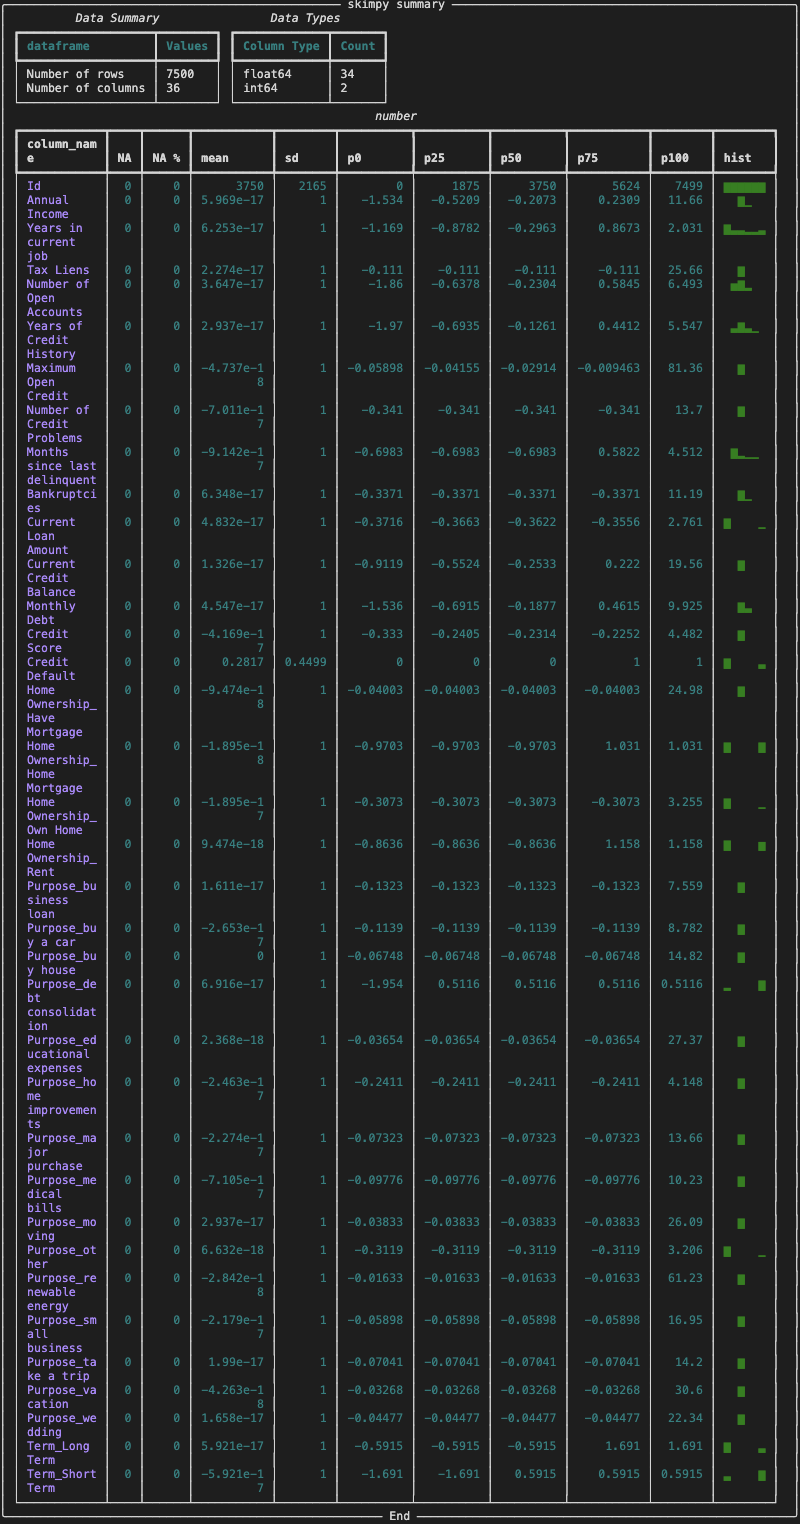
\includegraphics[width=0.5\textwidth]{figures/Annexe3.png}
\caption{Résumé Statistique descriptive train.}
\label{fig:annexe3}
\end{figure}

\section*{Annexe 4}
\label{sec:annexe4}
\begin{figure}[H]
\centering
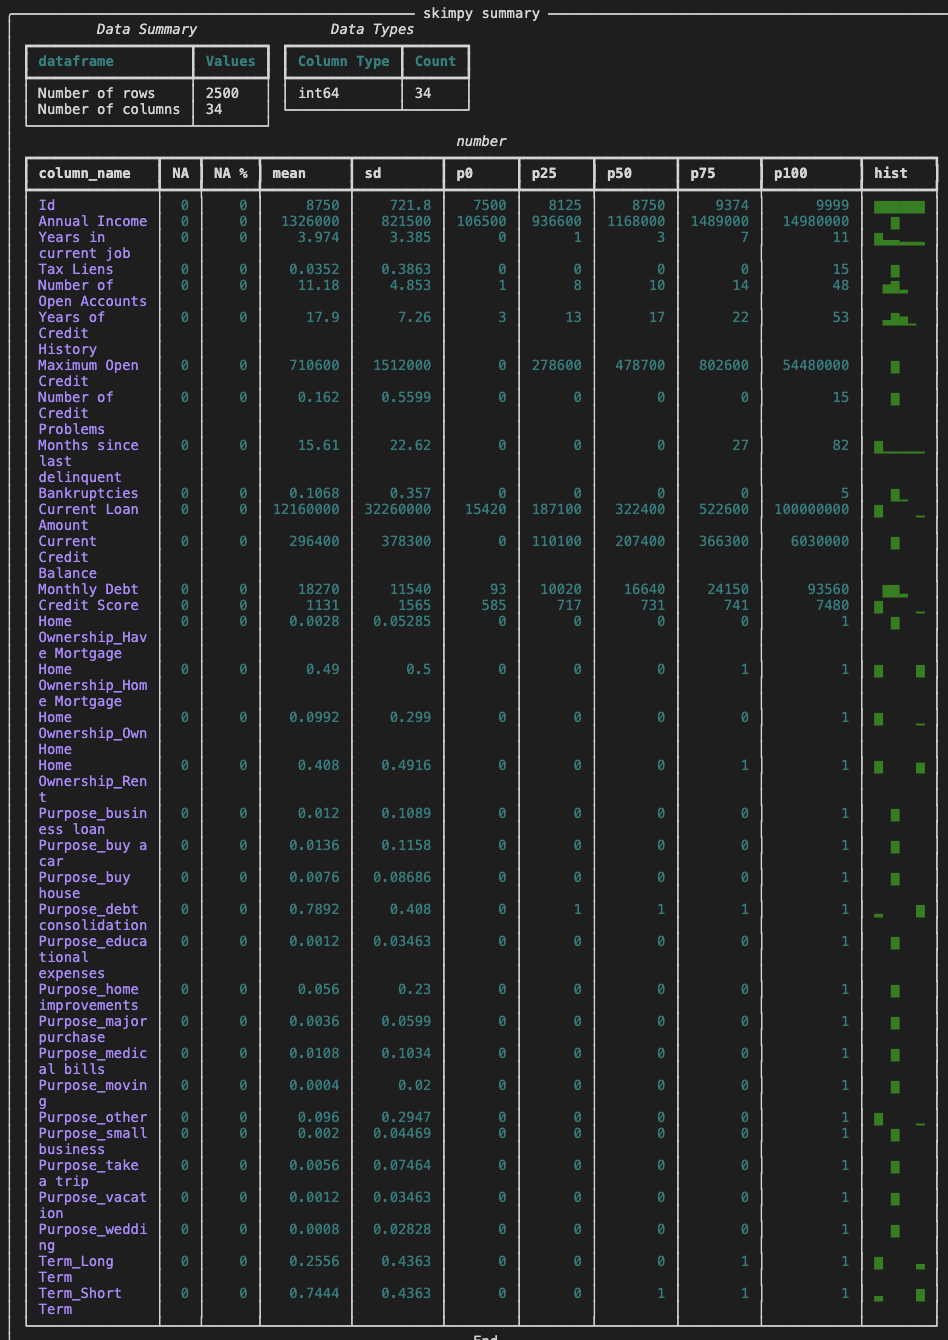
\includegraphics[width=1\textwidth]{figures/Annexe4.png}
\caption{Résumé Statistique descriptive jeu test.}
\label{fig:annexe4}
\end{figure}

\section*{Annexe 5}
\label{sec:annexe5}
\begin{figure}[H]
\centering
\includegraphics[width=1\textwidth]{figures/MatriceArbre.png}
\caption{Matrice de confusion Arbre de décision.}
\label{fig:annexe5}
\end{figure}


\begin{figure}[H]
\centering
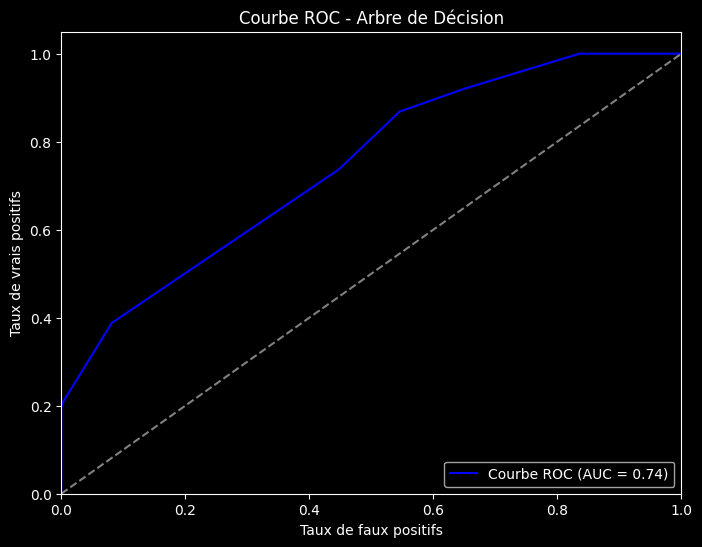
\includegraphics[width=1\textwidth]{figures/ROCArbre.png}
\caption{Courbe de ROC Arbre de décision.}
\end{figure}


\section*{Annexe 6}
\label{sec:annexe6}
\begin{figure}[H]
\centering
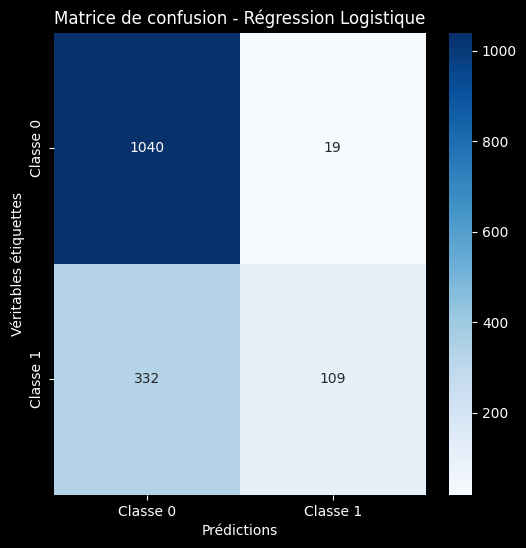
\includegraphics[width=1\textwidth]{figures/MatriceRL.png}
\caption{Matrice de confusion Régression logistique.}
\label{fig:annexe6}
\end{figure}


\begin{figure}[H]
\centering
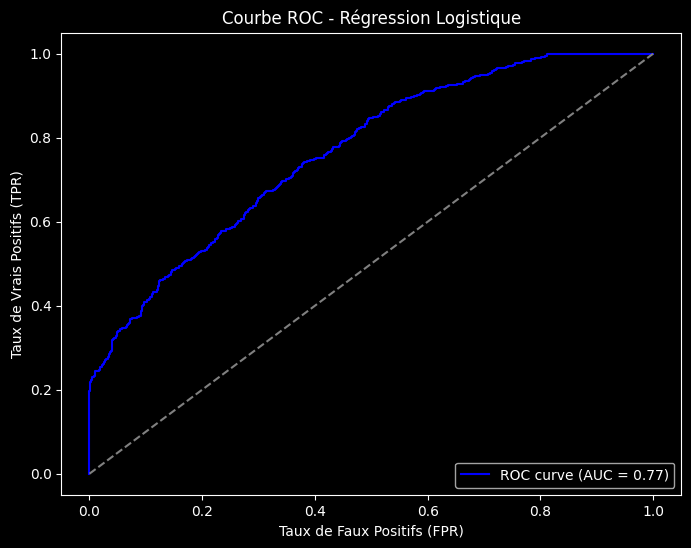
\includegraphics[width=1\textwidth]{figures/ROCRL.png}
\caption{Courbe de ROC Régression Logistique.}
\end{figure}

\section*{Annexe 7}
\label{sec:annexe7}
\begin{figure}[H]
\centering
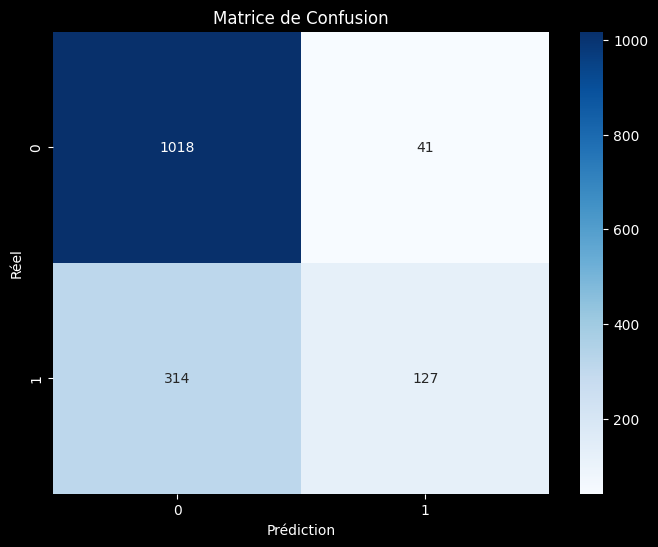
\includegraphics[width=1\textwidth]{figures/MatriceFoAl.png}
\caption{Matrice de confusion Forêt Aléatoire.}
\label{fig:annexe7}
\end{figure}


\begin{figure}[H]
\centering
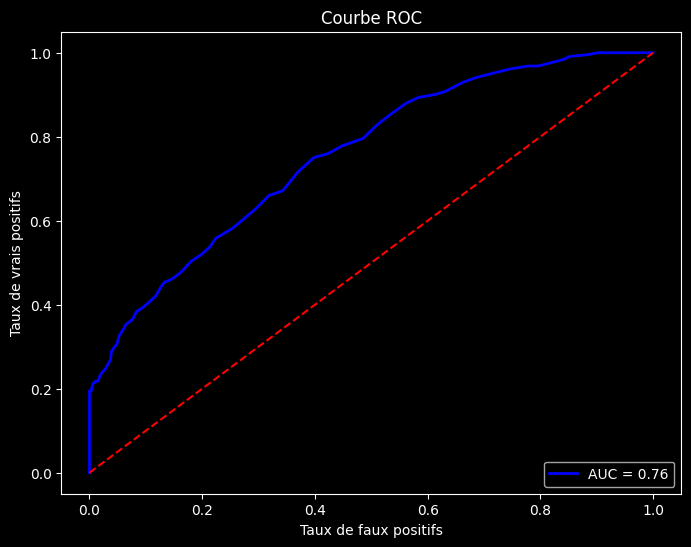
\includegraphics[width=1\textwidth]{figures/ROCAL.png}
\caption{Courbe de ROC Forêt Aléatoire}
\end{figure}

\section*{Annexe 8}
\label{sec:annexe8}
\begin{figure}[H]
\centering
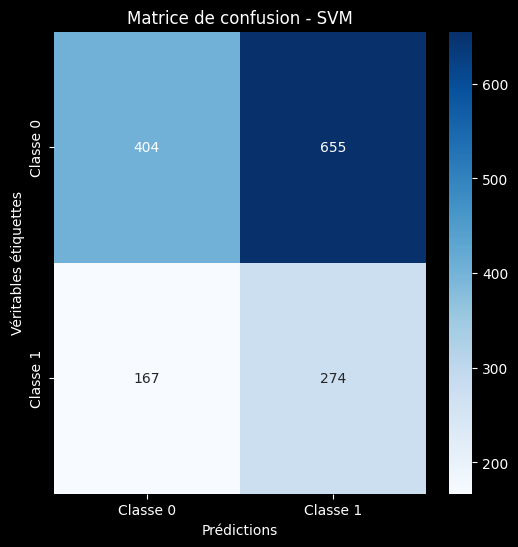
\includegraphics[width=1\textwidth]{figures/MatriceSVM.png}
\caption{Matrice de confusion SVM.}
\label{fig:annexe8}
\end{figure}


\begin{figure}[H]
\centering
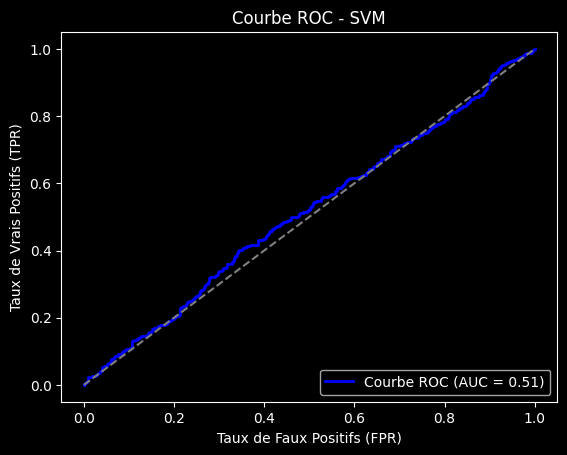
\includegraphics[width=1\textwidth]{figures/ROCSVM.png}
\caption{Courbe de ROC SVM.}
\end{figure}

\section*{Annexe 9}
\label{sec:annexe9}
\begin{figure}[H]
\centering
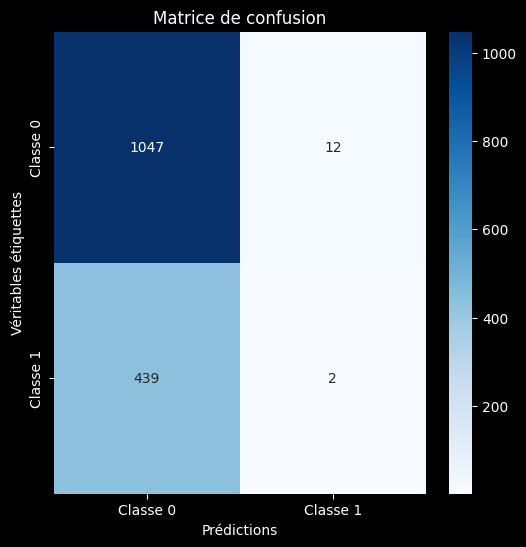
\includegraphics[width=1\textwidth]{figures/MatriceKNN.png}
\caption{Matrice de confusion KNN.}
\label{fig:annexe9}
\end{figure}


\begin{figure}[H]
\centering
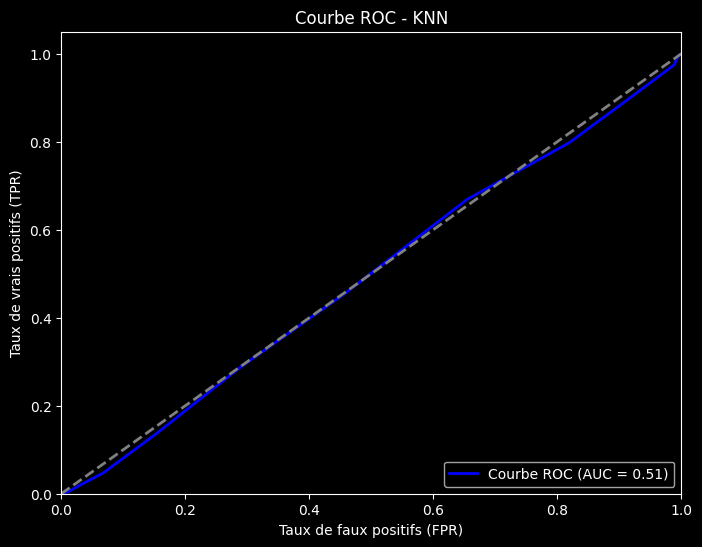
\includegraphics[width=1\textwidth]{figures/ROCKNN.png}
\caption{Courbe de ROC KNN.}
\end{figure}
\section*{Annexe 10}
\label{sec:annexe10}
\begin{figure}[H]
\centering
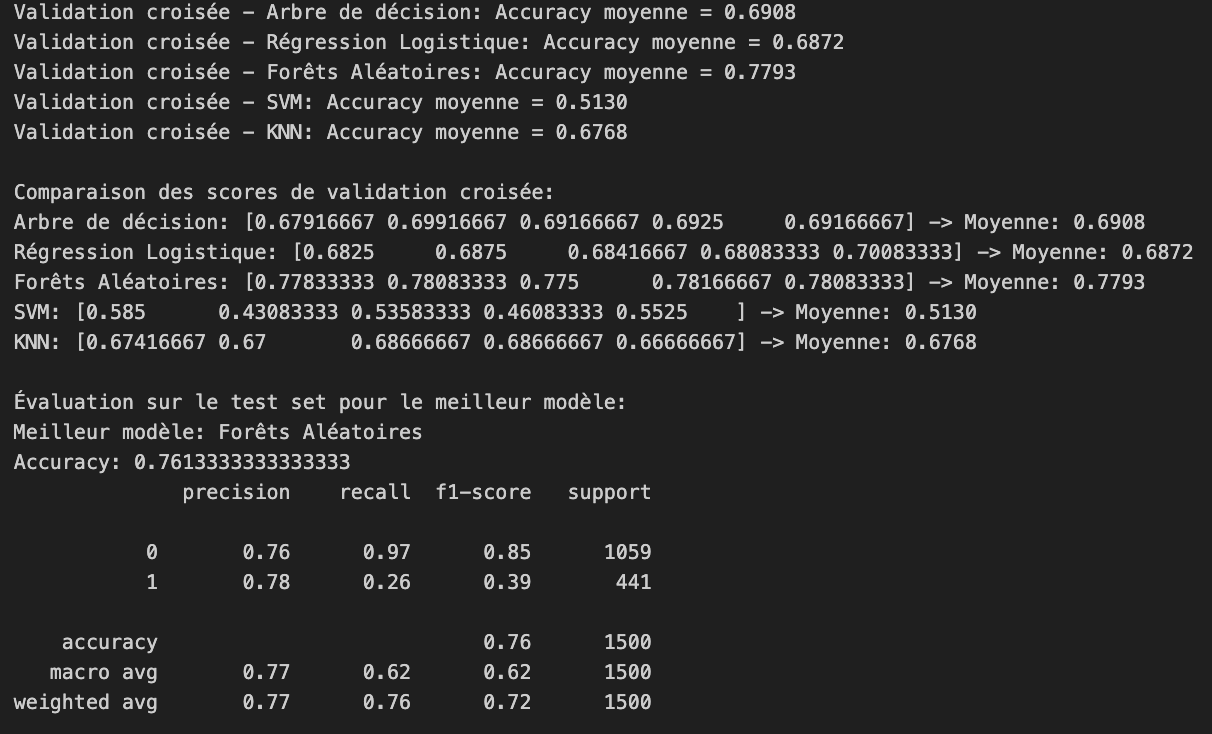
\includegraphics[width=1\textwidth]{figures/Annexe10.png}
\caption{Métrique Validation Forêt Aléatoire.}
\label{fig:annexe10}
\end{figure}

\begin{figure}[H]
\centering
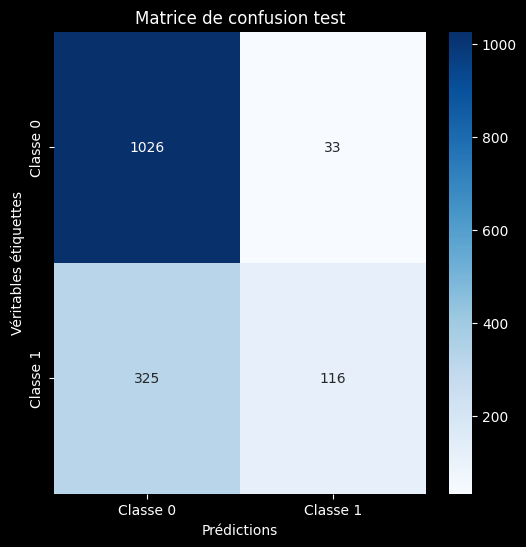
\includegraphics[width=1\textwidth]{figures/MatriceVC1.png}
\caption{Matrice de validation croisée Forêt Aléatoire.}
\end{figure}


\section*{Annexe 11}
\label{sec:annexe11}
\begin{figure}[H]
\centering
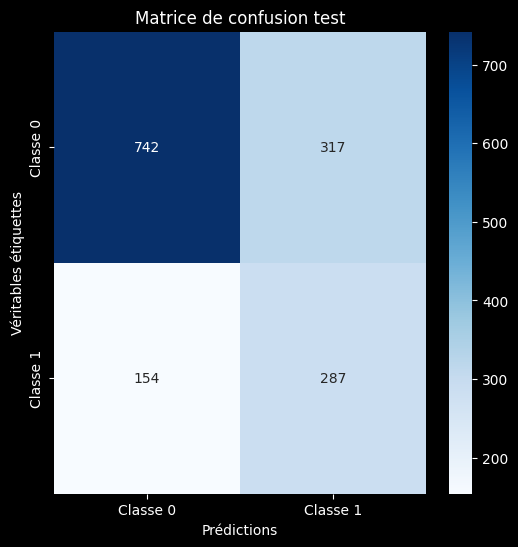
\includegraphics[width=1\textwidth]{figures/MatriceValANNEXE11.png}
\caption{Matrice de validation croisée Régression Logistique.}
\label{fig:annexe11}
\end{figure}
 
\addstarredchapter{Bibliographie}
\bibliographystyle{unsrt}
\bibliography{references}
\end{document}